\chapter{Testen der Ergebnisse}
\label{kap6}

Dieses Kapitel testet die Implementierung des nach \ac{ROS} und Gazebo migrierten Laufplaners. Zum einen können die Ergebnisse durch die Visualisierung in Gazebo überprüft werden. Eine weitere Möglichkeit der Auswertung, welche sich auch zur Fehleranalyse eignet, ist die Nutzung eines Frameworks, um mathematische Darstellungen anzufertigen. Dazu nutzt diese Arbeit das auf Python basierende Framework matplotlib \autocite{barrett2005matplotlib}. Dieses wird mit Hilfe einem Header für C++ eingebunden, welcher die Befehle im Hintergrund in Python ausführt. Damit lassen sich unter anderem Bewegungen der Füße und des Roboterkörpers in einem Graphen darstellen.

Das Random Sampling erfolgt wie in \autoref{kap3} beschrieben. Dabei gibt es einige Schritte, die bei der Implementierung fehlerhaft sein können, da sie auf verschiedenen Robotern mit anderen Werten ablaufen müssen. 

\begin{figure}[t!]
  \centering
  \begin{subfigure}[b]{.5\linewidth}
    \centering
    \includegraphics[scale=0.45]{kapitel5/footdownSuccess1}
    \subcaption{Direkte Suche}\label{kap5:footDownNormal1}
  \end{subfigure}%
  \begin{subfigure}[b]{.5\linewidth}
    \centering
    \includegraphics[scale=0.45]{kapitel5/footdownSuccess2}
    \subcaption{Direkte Suche}\label{kap5:footDownNormal2}
  \end{subfigure}\\
  \\[\smallskipamount]
  \begin{subfigure}[b]{.5\linewidth}
    \centering
    \includegraphics[scale=0.45]{kapitel5/footdownnoSuccess1}
    \subcaption{Spiralsuche}\label{kap5:footDownSpiral1}
  \end{subfigure}%
  \begin{subfigure}[b]{.5\linewidth}
    \centering
    \includegraphics[scale=0.45]{kapitel5/footdownnoSuccess2}
    \subcaption{Spiralsuche}\label{kap5:footDownSpiral2}
  \end{subfigure}%
  \caption{Auswertung der Positionsfindung beim Absetzen eines Fußes}
  \label{kap5:footDown}
\end{figure}

Die erste Herausforderung ist das Absetzen eines Fußes. Während das Anheben eines Fußes in der Regel immer möglich ist, kann es beim Absetzen zu Problemen kommen. Das Ziel ist es, den Fuß in eine neue gültige und zufällige Position zu bringen. Diese sollte nach Möglichkeit in Richtung Ziel liegen, damit der Roboter voranschreiten kann. Bei der Generierung der Position wird ausgehend von einer Startposition ein Vektor addiert, der leicht in Richtung Ziel verschoben ist. Danach wird ein weiterer zufälliger Vektor addiert. Dann wird versucht, den Fuß an dieser Stelle abzusetzen. Ist diese Position nicht gültig, wird mit Hilfe einer Spiralsuche eine bessere Position gesucht. Die Implementierung erforderte im Gegensatz zum Lauron andere Werte für Vektorlänge und den Abständen der Spiralsuche, um genau solche Positionen zu finden, die den Roboter besser zum Ziel bringen können.

Sind diese Werte angepasst, ergeben sich wie in \autoref{kap5:footDownNormal1} und \autoref{kap5:footDownNormal2} in den meisten Fällen bereits gültige Fußpositionen, ohne die Spiralsuche anwenden zu müssen, vorausgesetzt das Weltmodell ist flach. Selten kommt es dazu, dass eine Spiralsuche durchgeführt werden muss. Beim Ablauf der Sprialsuche wird wie in \autoref{kap5:footDownSpiral1} und \autoref{kap5:footDownSpiral2} in der Regel immer ein gültiges Ergebnis gefunden. Nur sehr selten kommt es vor, dass ein Fuß keine Absetzposition findet. Ist dies der Fall, soll der Algorithmus die generierte Lösung verwerfen.

\begin{figure}[b!]
    \begin{center}
    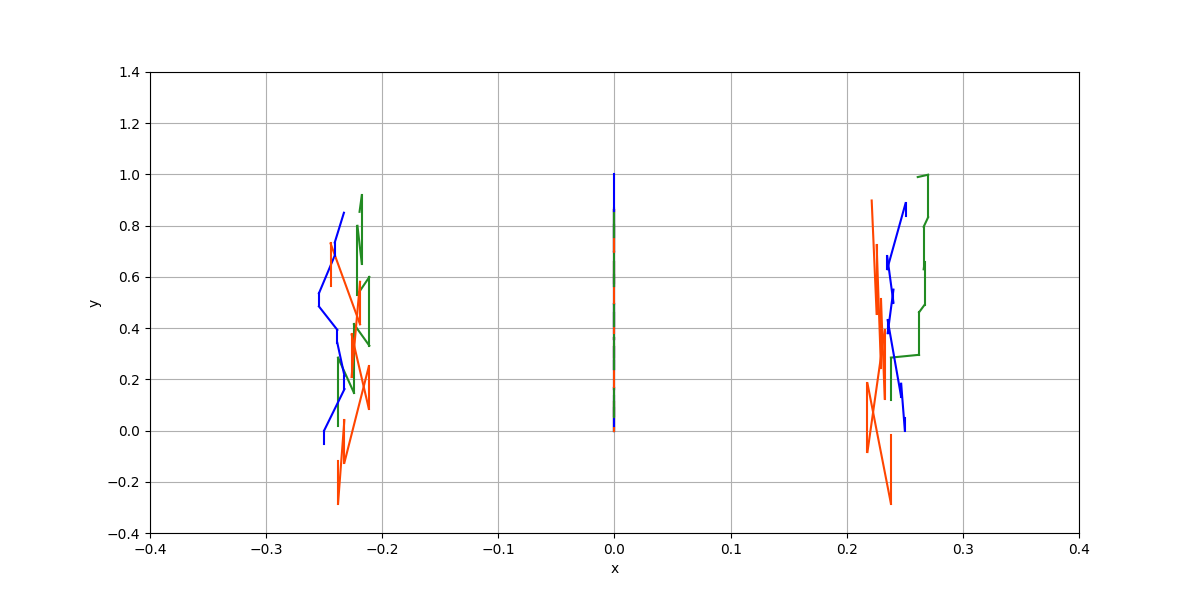
\includegraphics[width=0.94\textwidth]{kapitel5/footmov1}\hfill
    \\[\smallskipamount]
    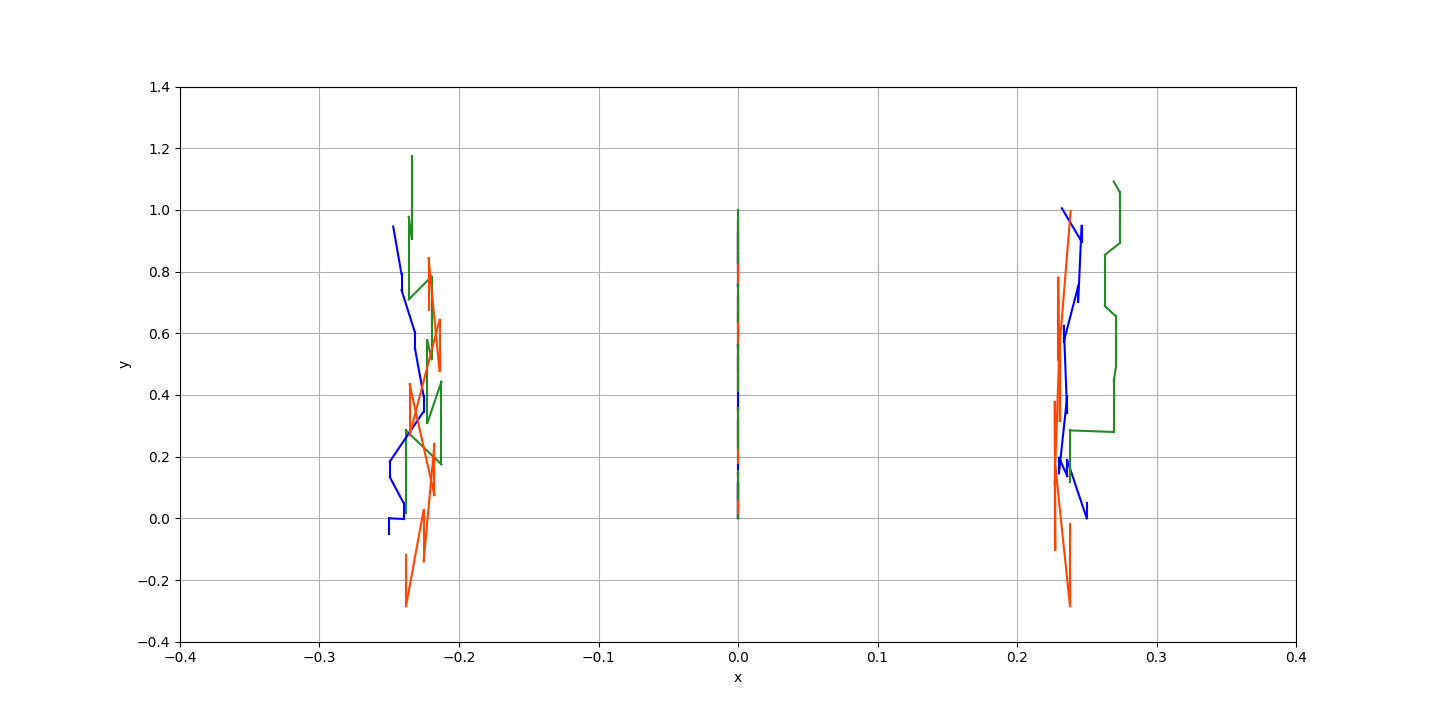
\includegraphics[width=0.94\textwidth]{kapitel5/footmov2}\hfill
    \\[\smallskipamount]
    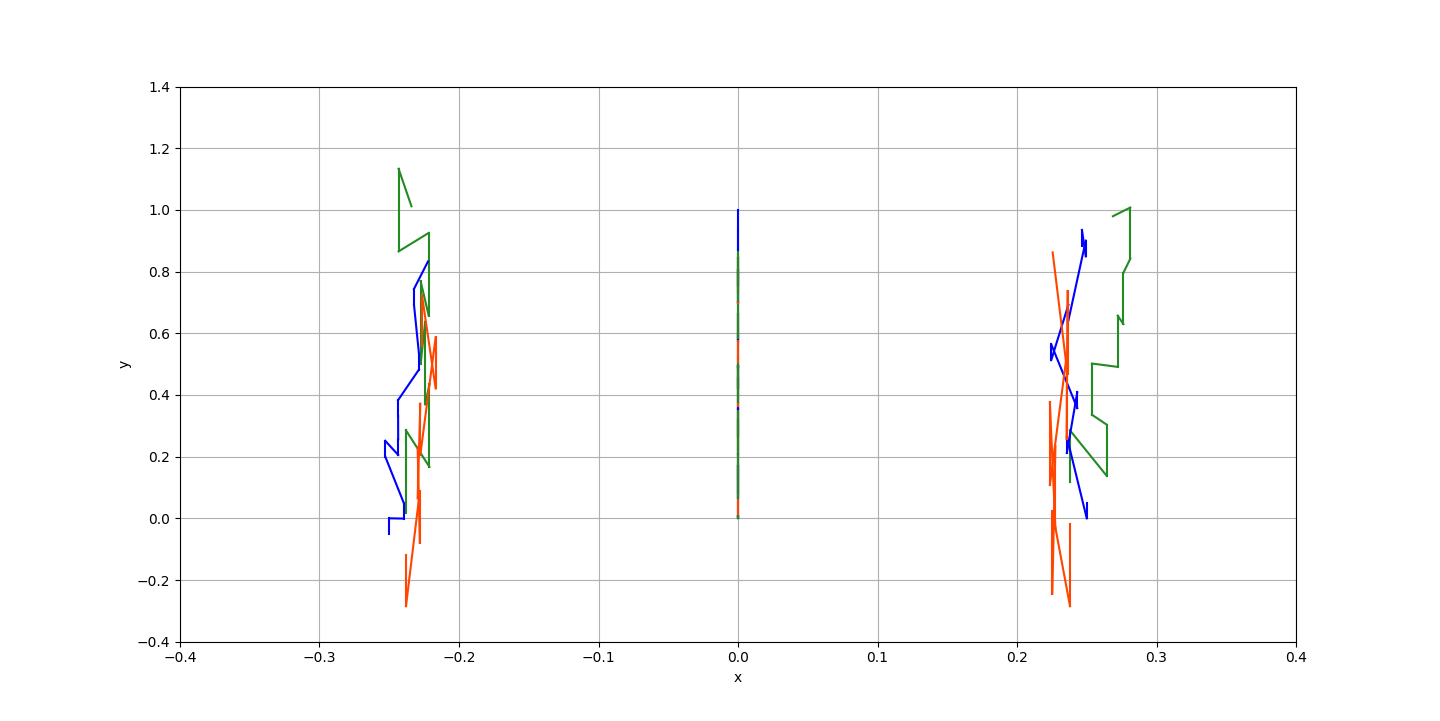
\includegraphics[width=0.94\textwidth]{kapitel5/footmov3}\hfill
    \caption{Auswertung von Bewegungen von Körper und Füßen}\label{kap5:footCenterMovements}
    \end{center}
\end{figure}

Eine weitere Herausforderung ist es, ob der Algorithmus es insgesamt schafft, gültige Lösungen zur anvisierten Zielposition zu generieren. In folgendem Beispiel versucht der Laufplaner für den Akrobat gültige Lösungen für die Bewegung von der Startposition $S(0,0)$ zur Zielposition $Z(0,1)$ zu generieren. Dies entspricht der Bewegungen von einem Meter. Dazu wird eine vollständig flache Welt genutzt. \autoref{kap5:footCenterMovements} zeigt drei nacheinander ausgeführte Generierungen von Lösungen für dieses Problem. Ferner zeigt es die einzelnen Fußbewegungen sowie die möglichen Bereiche, in denen sich die Körpermitte bewegen darf. Das Resultat ist in allen drei Fällen erfolgreich. Dass dies funktioniert, bestätigt ebenfalls, dass die Auswahl der nächsten Fußänderung, also die Entscheidung welcher Fuß angehoben oder abgesetzt wird, mittels der Glücksradauswahl geeignete Entscheidungen trifft, die nicht dafür sorgen, dass die Bewegungen sich gegenseitig aufheben.